%!TEX root = ../main.tex



\subsection{Overall Evaluation}\label{exp:sec:overall}

\begin{table}
	\centering
	\caption{Human cost of different methods}
	\vspace{-1.2em}
	\small
	\begin{tabular}{cccc}
		\hline
		Dataset & $\seven$ & $\three$ & $\one$\\
		\hline
		\nursery & 37 & 22 & 3278\\
		\hr & 44 & 32 & 5475\\
		\adult & 63 & 81 & 10752\\
		\credit & 52 & 67 & -\\
		\bike & 38 & 25 & -\\
		\air & 98 & 102 & -\\
		\hline
	\end{tabular}
	\label{tbl:humancost}
	\vspace{-1em}
\end{table}





In this part, we compare \ours solutions with baselines. We use $\rho = \frac{K}{|\train|}$ to denote the proportion of coreset  to the entire train set.  %\cc{
We set  $\rho=0.005$ for datasets (1)-(4), $\rho=0.001$ and  $\rho=0.0005$ for larger datasets (5) and (6) respectively.
%}
 We  will further  conduct evaluation by varying the coreset size  in Section~\ref{exp:sec:end2end}.







%\begin{figure}[!h]
%	\centering
%	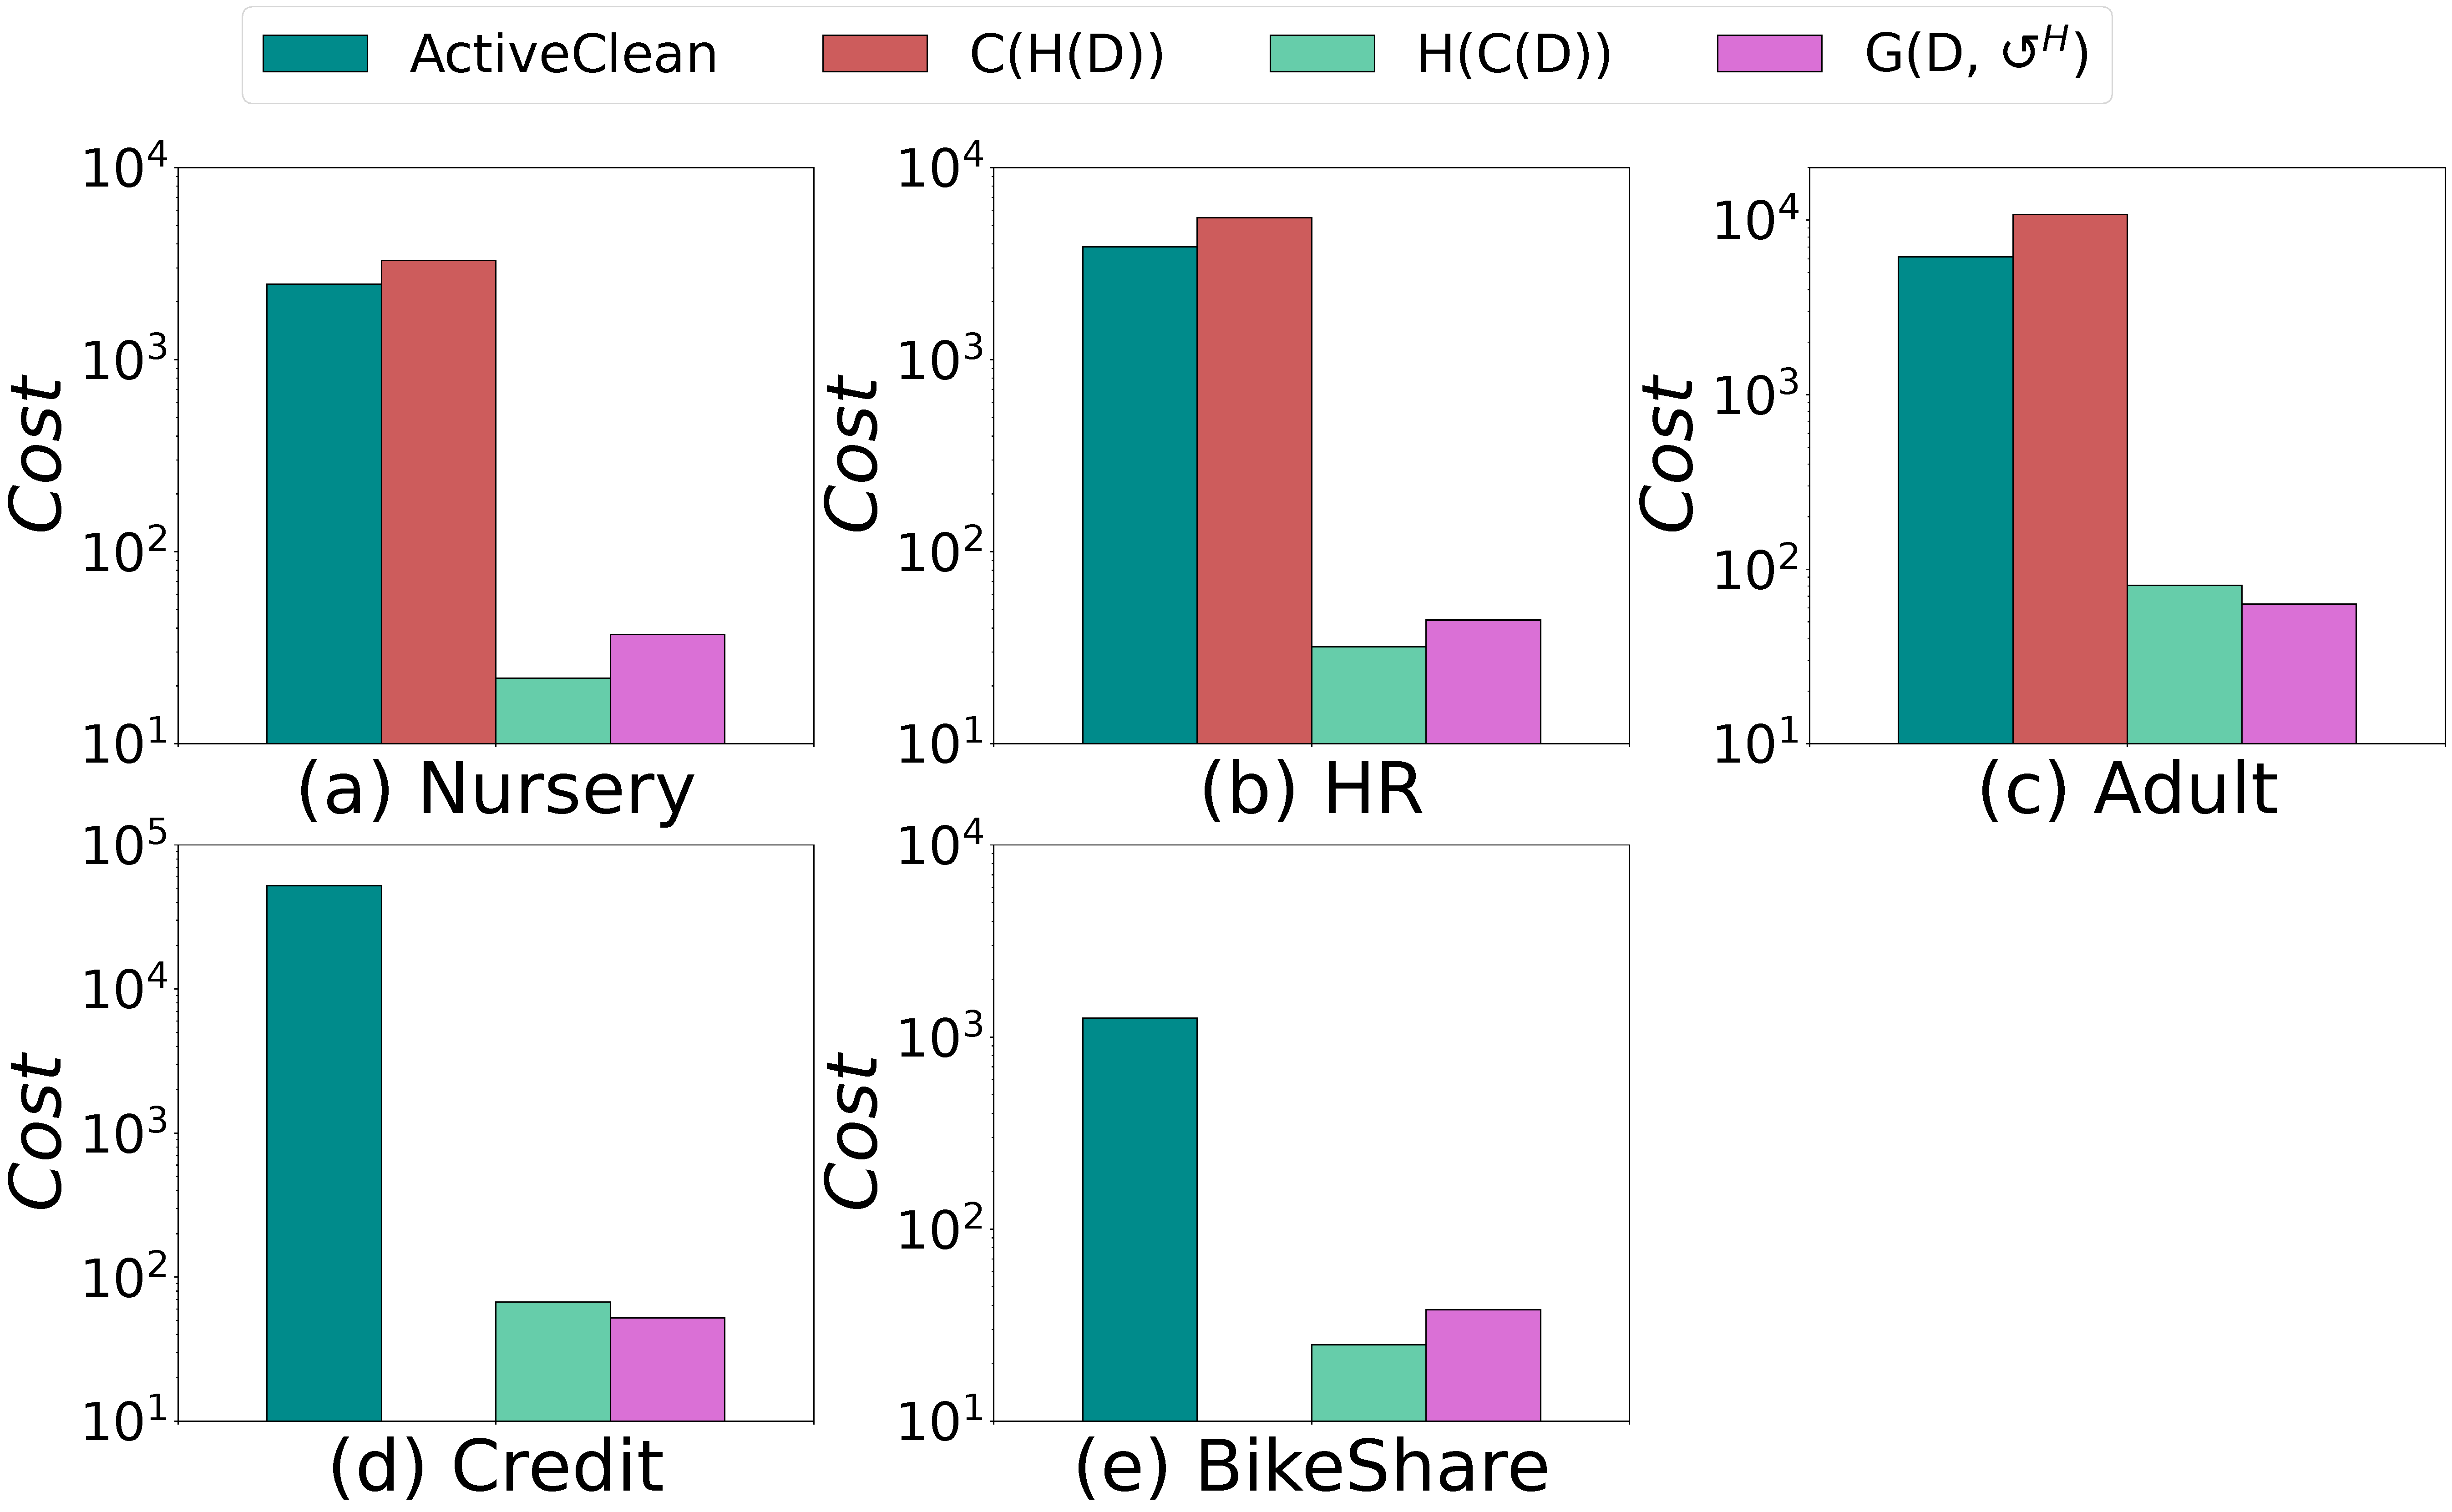
\includegraphics[width=\columnwidth]{figs/humancost}
%	\vspace{-2em}
%	\caption{Human cost of \ours.}
%	\label{fig:humancost}
%\end{figure}


%\noindent{\bf Evaluation of model accuracy.}
\subsubsection{Evaluation of model accuracy.}
The results are provided in Figure~\ref{fig:effectiveness}. To summarize, the result could be generally ranked as $\seven/\one/\truth > $ $\eight/\boostclean/\gain$ > $\two$ > $\mixcore$ > $\actclean$ > $\three/\four$ > $\noclean$.
Next, we explain the results.

In general, on all datasets, our method $\seven$, \truth~ and $\one$~   perform the best. 
 \truth~ and $\one$ achieve a high accuracy because they ask the human to impute missing values accurately, but incur a high human cost.  For example, \truth~and $\one$ achieve accuracy of 71.9\% and 71.7\% on \adult. $\seven$  is competitive with them because it selects a good coreset that can well represent the unknown ground truth via gradient approximation. In addition, we can observe that $\seven$ performs better than $\eight$ because human imputation is more accurate than automatic methods. For example, on \adult, $\seven$ has an accuracy of 71.7\%, while $\eight$ and others are below 68\%. $\eight$, \boostclean and \gain have competitive performance on accuracy. \boostclean and \gain can have a not bad performance because they impute all tuples and train on the entire dataset, but they cannot achieve efficient training (see \ref{sec:exp:efficiency}). But  we can train on the much smaller coreset generated by $\eight$ with a good accuracy, because \ours considers the possible repairs to derive the coreset  that can approximate the full gradient of the entire dataset. Given the same number of tuples to be imputed by human,  $\seven$ also outperforms \actclean because we have theoretical guarantees on the gradient approximation. 
 %For example, on dataset \adult, $\eight$ has an accuracy of 69.8\%, which is better than that of \boostclean (65.8\%), \actclean (63.9\%) and \gain (65.1\%). Our method $\eight$ outperforms \boostclean because we consider possible repairs and the gradients of tuples in our algorithm.   \actclean also considers gradients of tuples, which prioritizes imputing tuples that much influence the model gradients, but they use heuristics to estimate the influence, which is not accurate enough. \gain does not perform well because it does not much consider possible repairs and not impute the tuple considering the downstream model performance.
  For other baselines,  $\three$ and $\four$ do not perform well because they select the coreset from an incomplete dataset.  $\two$ cannot achieve a good performance because the selected coreset can not well represent the complete entire dataset, as it does not consider possible repairs as our method.  %it is hard for the automatic method to always achieve a high imputation accuracy. 
  {\mixcore} does not perform well (\eg 65.2\% on \adult) because $\seven$ and $\eight$ select a better coreset considering the full data. For \noclean, on  \adult, the model  has an accuracy of 61.3\% because of the incomplete tuples.



 



\subsubsection{Evaluation of the efficiency.}~\label{sec:exp:efficiency} We  evaluate the efficiency of all methods, including the machine cost and human cost.

\noindent{\bf Machine cost.} Machine cost is shown  in Figure~\ref{fig:efficiency}.  The results could be ranked as $\three/\four/\seven/\eight/\one/\mixcore < \two < \truth < \noclean < \actclean < \boostclean/\gain$. We can observe that the first 5 methods in the ranking have low machine cost, mainly because they train based on the selected coreset and do not need iterative training. $\seven$ and  $\eight$ are slightly slower  because they need to iterate several possible repairs during the process of coreset selection.  But $\seven$ is still more efficient than \noclean, \truth, \boostclean and \gain by more than one order of magnitude,  because they need to train on the entire training data. 
 Moreover, \actclean~  and \boostclean are  not efficient either because they incorporate multiple training times, so as to estimate the gradient while data imputation. \gain is slow because training multiple imputation models takes time.


\noindent{\bf Human cost.} In terms of the human cost, $\one$, $\three$, $\seven$ and  \actclean~ involve human. As shown in~Table~\ref{tbl:humancost}, $\one$ is very expensive because it asks the human to impute all missing tuples. For example, on datset \adult, 10752 tuples have to be imputed. We do not compare \credit, \bike and \air for $\one$ because they do not have the ground truth.
 But $\three$ and $\seven$ are cost-effective because human just needs to impute missing tuples in the much smaller coreset. For example, they only cost 81 and 63 tuples on dataset \adult respectively. 
\actclean~ asks the human to iteratively impute the data. Given the same number of tuples to impute, our method can achieve much higher accuracy. We will  evaluate it in details in next subsection.
 



\noindent \textbf{Summary.} 
Based on the results, we have the following conclusions.
(1) Our proposed methods $\seven$ and $\eight$ can achieve high model accuracy because the selected coreset can well represent the underlying ground truth by gradient approximation considering possible repairs. Meanwhile, they are practical because of the low machine cost. (2) Compared with $\one$ that involves human to impute the entire dataset $D$, the human cost of $\seven$ is much lower, as observed in Table~\ref{tbl:humancost}, e.g., $37$ vs. $3278$ on the \nursery dataset. Thus, we can choose $\seven$ when we want to achieve high model accuracy and afford a certain human cost. (3) 
%Meanwhile, they are practical because of the low machine cost. Although $\seven$ needs human involvement, the human cost is also low. We can choose it when we want to achieve high model accuracy. 
If we neither care very much about the accuracy nor consider to incur human cost, the much more efficient $\eight$ is a good choice.



%Figure.~\ref{fig:humancost} shows the human cost of different methods. The results could be ranked as $\seven/\three \ll \actclean < \one$.

